\newpage

\subsection{QuizziPedia::Front-End::Views}
\subsubsection{Informazioni generali}
\label{QuizziPedia::Front-End::Views}
\begin{figure}
	\centering
	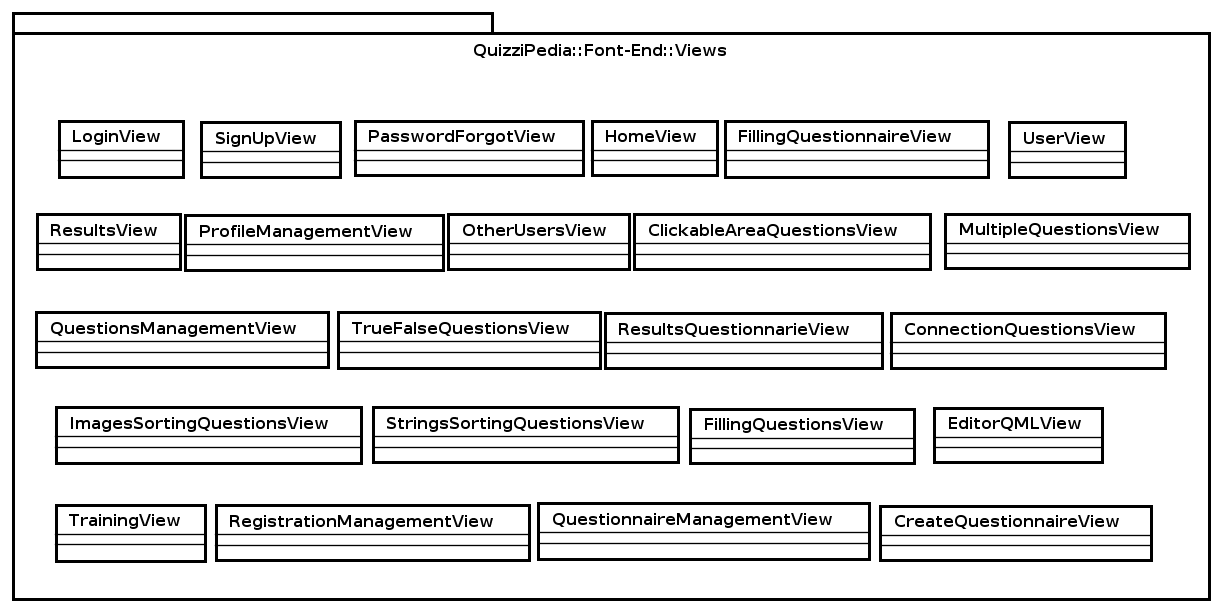
\includegraphics[scale=0.45]{UML/Package/QuizziPedia_Front-End_Views.png}
	\caption{QuizziPedia::Front-End::Views}
\end{figure}
\begin{itemize}
	\item \textbf{Descrizione}: package contenente le views front-end dell'applicazione;
	\item \textbf{Padre}: \texttt{Front-End}
	\item \textbf{Interazione con altri componenti}:
	\begin{itemize}
		\item \texttt{Controllers}: package contenente i controllers front-end dell'applicazione;
		\item \texttt{Directives}: package contenente le directives front-end dell'applicazione;
		\item \texttt{ModelViews}: package contenente le classi che saranno presenti nella variabile d'ambiente \texttt{\$scope} di \textit{Angular.js\ped{G}} che permettono il \textit{Two-Way Data-Binding\ped{G}} tra le views e i controllers;
		\item \texttt{Directives}: package contenente i templates front-end dell'applicazione.
	\end{itemize}
\end{itemize}
\subsubsection{Classi}


\paragraph{QuizziPedia::Front-End::Views::LoginView}
\begin{figure} [ht]
	\centering
	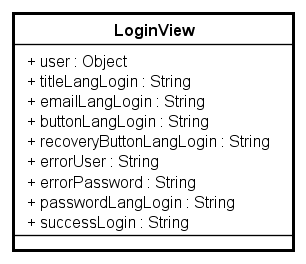
\includegraphics[scale=0.80]{UML/Classi/Front-End/QuizziPedia_Front-end_Views_LoginView.png}
	\caption{QuizziPedia::Front-End::Views::LoginView}
\end{figure} \FloatBarrier
\begin{itemize}
	\item \textbf{Descrizione}: view contenente le form necessarie per effettuare il login. Contiene inoltre un link alla pagina di registrazione e uno alla pagina per il recupero della password;
	\item \textbf{Utilizzo}: premette all'utente di autenticarsi inserendo username e password;
	\item \textbf{Relazioni con altre classi}:
	\begin{itemize}
		\item \textit{IN} \texttt{LoginController}: questa classe permette di gestire l'autenticazione dell'utente al sistema;
		\item \textit{IN} \texttt{LoginModelView}: classe di tipo modelview la cui istanzazione è contenuta all'interno della variabile di ambiente \$scope di \texttt{Angular.js}. All'interno di essa sono presenti le variabili e i metodi necessari per il \textit{Two-Way Data-Binding\ped{G}} tra la view \texttt{LoginView} e il controller \texttt{LoginController};
		\item \textit{IN} \texttt{LangModel}: rappresenta il modello delle informazioni per la giusta traduzione dell'applicazione.
	\end{itemize}
	\item \textbf{Attributi}:
	\begin{itemize}
		\item \texttt{+ user: Object} \\ Campo dati contenente due attributi: \texttt{email} e \texttt{password};
		\item \texttt{+ titleLang: String} \\ Attributo che viene utilizzato per visualizzare la giusta traduzione del titolo della pagina, in italiano o in inglese;
		\item \texttt{+ usernameLang: String} \\ Attributo che viene utilizzato per visualizzare la giusta traduzione della \textit{label\ped{G}} per l'inserimento del nome utente, in italiano o in inglese; 
		\item \texttt{+ buttonLoginLang: String} \\ Attributo che viene utilizzato per visualizzare la giusta traduzione della \textit{label\ped{G}} per il bottone di autenticazione, in italiano o in inglese;
		\item \texttt{+ recoveryBottonLang: String} \\ Attributo che viene utilizzato per visualizzare la giusta traduzione della \textit{label\ped{G}} per il bottone di link al recupero della password, in italiano o in inglese;
		\item \texttt{+ successLogin: String} \\ Attributo che visualizza un messaggio di avvenuta registrazione;
		\item \texttt{+ errorUser: String} \\ Attributo che visualizza un eventuale messaggio di errore nell'inserimento della username, in italiano o in inglese;
		\item \texttt{+ errorPassword: String} \\ Attributo che visualizza un eventuale messaggio di errore nell'inserimento della password, in italiano o in inglese.
	\end{itemize}
\end{itemize}


\paragraph{QuizziPedia::Front-End::Views::SignUpView}
\begin{figure} [ht]
	\centering
	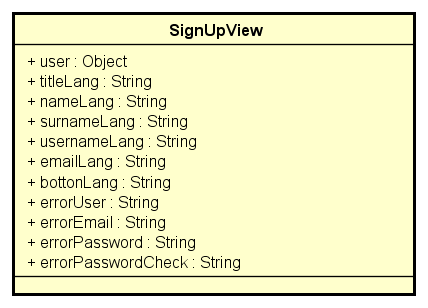
\includegraphics[scale=0.80]{UML/Classi/Front-End/QuizziPedia_Front-end_Views_SignUpView.png}
	\caption{QuizziPedia::Front-End::Views::SignUpView}
\end{figure} \FloatBarrier
\begin{itemize}
	\item \textbf{Descrizione}: view contenente le form dedicate alla registrazione utente. Contiene inoltre un link alla pagina di login;
	\item \textbf{Utilizzo}: permette all'utente di registrarsi al sistema inserendo i campi dati necessari;
	\item \textbf{Relazioni con altre classi}:
	\begin{itemize}
		\item \textit \texttt{SignUpController}: questa classe permette di gestire la registrazione di un utente al sistema;
		\item \textit{IN} \texttt{SignUpModelView}: classe di tipo modelview la cui istanzazione è contenuta all'interno della variabile di ambiente \$scope di \texttt{Angular.js}. All'interno di essa sono presenti le variabili e i metodi necessari per il \textit{Two-Way Data-Binding\ped{G}} tra la view \texttt{SignUpView} e il controller \texttt{SignUpController};
		\item \textit{IN} \texttt{LangModel}: rappresenta il modello delle informazioni per la giusta traduzione dell'applicazione.
	\end{itemize}
	\item \textbf{Attributi}:
	\begin{itemize}
		\item \texttt{+ user: Object} \\ Campo dati contenente i seguenti attributi: \texttt{name}, \texttt{surname}, \texttt{username}, \texttt{email}, \texttt{password} e \texttt{passwordCheck};
		\item \texttt{+ titleLang: String} \\ Attributo che viene utilizzato per visualizzare la giusta traduzione del titolo della pagina, in italiano o in inglese;
		\item \texttt{+ nameLang: String} \\ Attributo che viene utilizzato per visualizzare la giusta traduzione della \textit{label\ped{G}} per l'inserimento del nome, in italiano o in inglese;
		\item \texttt{+ surnameLang: String} \\ Attributo che viene utilizzato per visualizzare la giusta traduzione della \textit{label\ped{G}} per l'inserimento del cognome, in italiano o in inglese;
		\item \texttt{+ usernameLang: String} \\ Attributo che viene utilizzato per visualizzare la giusta traduzione della \textit{label\ped{G}} per l'inserimento del nome utente, in italiano o in inglese;
		\item \texttt{+ emailLang: String} \\ Attributo che viene utilizzato per visualizzare la giusta traduzione della \textit{label\ped{G}} per l'inserimento della posta elettronica, in italiano o in inglese;
		\item \texttt{+ buttonSignUpLang: String} \\ Attributo che viene utilizzato per visualizzare la giusta traduzione della \textit{label\ped{G}} per il bottone di registrazione, in italiano o in inglese;
		\item \texttt{+ loginButtonLang: String} \\ Attributo che viene utilizzato per visualizzare la giusta traduzione della \textit{label\ped{G}} per il bottone di link all'autenticazione, in italiano o in inglese;
		\item \texttt{+ successSignUp: String} \\ Attributo che visualizza un messaggio di avvenuta registrazione;
		\item \texttt{+ errorUser: String} \\ Attributo che visualizza un eventuale messaggio di errore nell'inserimento della username;
		\item \texttt{+ errorEmail: String} \\ Attributo che visualizza un eventuale messaggio di errore nell'inserimento della email;
		\item \texttt{+ errorPassword: String} \\ Attributo che visualizza un eventuale messaggio di errore nell'inserimento della password;
		\item \texttt{+ errorPasswordCheck: String} \\ Attributo che visualizza un eventuale messaggio di errore nell'inserimento della password di conferma.
	\end{itemize}
\end{itemize}


\paragraph{QuizziPedia::Front-End::Views::PasswordForgotView}
\begin{figure} [ht]
	\centering
	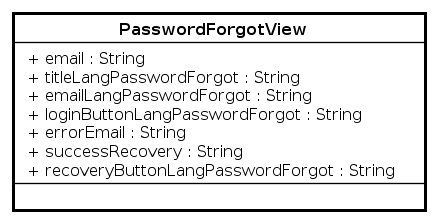
\includegraphics[scale=0.80]{UML/Classi/Front-End/QuizziPedia_Front-end_Views_PasswordForgotView.png}
	\caption{QuizziPedia::Front-End::Views::PasswordForgotView}
\end{figure} \FloatBarrier
\begin{itemize}
	\item \textbf{Descrizione}: view contenente le form necessarie per il recupero della password dimenticata;
	\item \textbf{Utilizzo}: permette all'utente di recuperare la password dimenticata inserendo i campi dati necessari;
	\item \textbf{Relazioni con altre classi}:
	\begin{itemize}
			\item \textit{IN} \texttt{PasswordForgotController}: questa classe permette di gestire il ripristino della password dimenticata;
			\item \textit{IN} \texttt{PasswordForgotModelView}: classe di tipo modelview la cui istanzazione è contenuta all'interno della variabile di ambiente \$scope di \texttt{Angular.js}. All'interno di essa sono presenti le variabili e i metodi necessari per il \textit{Two-Way Data-Binding\ped{G}} tra la view \texttt{PasswordForgotView} e il controller \texttt{PasswordForgotController};
			\item \textit{IN} \texttt{LangModel}: rappresenta il modello delle informazioni per la giusta traduzione dell'applicazione.
	\end{itemize}
	\item \textbf{Attributi}:
	\begin{itemize}
		\item \texttt{+ user: Object} \\ Campo dati contenente l'attributo \texttt{email};
		\item \texttt{+ titleLang: String} \\ Attributo che viene utilizzato per visualizzare la giusta traduzione del titolo della pagina, in italiano o in inglese;
		\item \texttt{+ emailLang: String} \\ Attributo che viene utilizzato per visualizzare la giusta traduzione della \textit{label\ped{G}} per l'inserimento della posta elettronica, in italiano o in inglese;
		\item \texttt{+ loginButtonLang: String} \\ Attributo che viene utilizzato per visualizzare la giusta traduzione della \textit{label\ped{G}} per il bottone di link all'autenticazione, in italiano o in inglese;
		\item \texttt{+ successRecovery: String} \\ Attributo che visualizza un messaggio di avvenuto invio della nuova password;
		\item \texttt{+ errorEmail: String} \\ Attributo che visualizza un eventuale messaggio di errore nell'inserimento della email.
	\end{itemize}
\end{itemize}


\paragraph{QuizziPedia::Front-End::Views::HomeView}
\begin{figure} [ht]
	\centering
	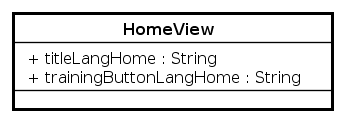
\includegraphics[scale=0.80]{UML/Classi/Front-End/QuizziPedia_Front-end_Views_HomeView.png}
	\caption{QuizziPedia::Front-End::Views::HomeView}
\end{figure} \FloatBarrier
\begin{itemize}
	\item \textbf{Descrizione}: view contenente la direttiva per barra di ricerca degli utenti e questionari e il bottone che porterà l'utente nella modalità allenamento;
	\item \textbf{Utilizzo}: viene utilizzata come view iniziale dell'applicazione;
	\item \textbf{Relazioni con altre classi}:
	\begin{itemize}
		\item \textit{IN} \texttt{HomeController}: questa classe permette di gestire la home page;
		\item \textit{IN} \texttt{HomeModelView}: classe di tipo modelview la cui istanzazione è contenuta all'interno della variabile di ambiente \$scope di \texttt{Angular.js}. All'interno di essa sono presenti le variabili e i metodi necessari per il \textit{Two-Way Data-Binding\ped{G}} tra la view \texttt{HomeView} e il controller \texttt{HomeController};
		\item \textit{IN} \texttt{SearchDirective}: directive che permette di effettuare la ricerca di utenti e questionari;
		\item \textit{IN} \texttt{LangModel}: rappresenta il modello delle informazioni per la giusta traduzione dell'applicazione.
	\end{itemize}
	\item \textbf{Attributi}:
	\begin{itemize}
		\item \texttt{+ titleLang: String} \\ Attributo che viene utilizzato per visualizzare la giusta traduzione del titolo della pagina, in italiano o in inglese;
		\item \texttt{+ trainingButtonLang: String} \\ Attributo che viene utilizzato per visualizzare la giusta traduzione della \textit{label\ped{G}} per il bottone di link all'autenticazione, in italiano o in inglese.
	\end{itemize}
\end{itemize}
	
	
\paragraph{QuizziPedia::Front-End::Views::ResultsView}
\begin{figure} [ht]
	\centering
	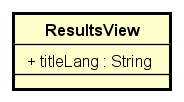
\includegraphics[scale=0.80]{UML/Classi/Front-End/QuizziPedia_Front-end_Views_ResultsView.png}
	\caption{QuizziPedia::Front-End::Views::ResultsView}
\end{figure} \FloatBarrier
\begin{itemize}
	\item \textbf{Descrizione}: view contenente i risultati della ricerca effettuata, sia gli utenti che i questionari trovati;
	\item \textbf{Utilizzo}: viene visualizzata dopo aver effettuato la ricerca di un utente o di un questionario nella barra di ricerca presente nella SearchDirective e permette di selezionare un risultato presente al suo interno; 
	\item \textbf{Relazioni con altre classi}:
	\begin{itemize}
		\item \textit{IN} \texttt{SearchController}: questa classe permette di gestire la ricerca di questionari e utenti all'interno dell'applicazione;
		\item \textit{IN} \texttt{ResultsModelView}: classe di tipo modelview la cui istanzazione è contenuta all'interno della variabile di ambiente \$scope di \texttt{Angular.js}. All'interno di essa sono presenti le variabili e i metodi necessari per il \textit{Two-Way Data-Binding\ped{G}} tra la view \texttt{ResultsView} e il controller \texttt{SearchController};
		\item \textit{IN} \texttt{SubscribeResultDirective}: directive che permette di visualizzare e iscriversi ai questionari ricercati;
		\item \textit{IN} \texttt{UserResultsDirective}: directive che permette di visualizzare la lista degli utenti ricercati dopo aver utilizzato l'apposita funzione di ricerca;
		\item \textit{IN} \texttt{LangModel}: rappresenta il modello delle informazioni per la giusta traduzione dell'applicazione.
	\end{itemize}
	\item \textbf{Attributi}:
		\begin{itemize}
			\item \texttt{+ titleLang: String} \\ Attributo che viene utilizzato per visualizzare la giusta traduzione del titolo della pagina, in italiano o in inglese.
		\end{itemize}
\end{itemize}


\paragraph{QuizziPedia::Front-End::Views::UserView}
\begin{figure} [ht]
	\centering
	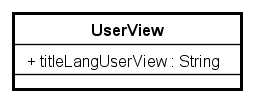
\includegraphics[scale=0.80]{UML/Classi/Front-End/QuizziPedia_Front-end_Views_UserView.png}
	\caption{QuizziPedia::Front-End::Views::UserView}
\end{figure} \FloatBarrier
\begin{itemize}
	\item \textbf{Descrizione}: view contenente le direttive dei dati personali dell'utente, delle sue statistiche relative ai questionari e agli allenamenti effettuati e dei questionari a cui è iscritto;
	\item \textbf{Utilizzo}:  permette ad un utente di visualizzare i propri dati personali e le proprie statistiche e di controllare a quali questionari è iscritto. 
	\item \textbf{Relazioni con altre classi}:
	\begin{itemize}
		\item \textit{IN} \texttt{StatisticsDirective}: directive che permette di visualizzare le statistiche di un utente;
		\item \textit{IN} \texttt{UserDetailsDirective}: directive che permette di visualizzare i dati personali di un utente;
		\item \textit{IN} \texttt{QuestionnaireDetailsDirective}: rappresenta il componente grafico che permette all'utente di visualizzare la lista di questionari che può compilare. Ogni item di questa lista contiene:
		\begin{itemize}
			\item Nome del questionario;
			\item Autore del questionario;
			\item Argomento del questionario;
			\item Parole chiave del questionario;
		\end{itemize}
		Al verificarsi dell'evento click su un item della lista l'utente verrà indirizzato alla view per la compilazione del questionario selezionato;
		\item \textit{IN} \texttt{QuestionnaireDetailsDoneDirective}: rappresenta il componente grafico che permette all'utente di visualizzare la lista di questionari che ha già compilato e di conseguenza vederne le valutazioni. Ogni item di questa lista contiene:
		\begin{itemize}
			\item Nome del questionario;
			\item Autore del questionario;
			\item Argomento del questionario;
			\item Parole chiave del questionario;
			\item Valutazione del questionario.
		\end{itemize}
		\item \textit{IN} \texttt{LangModel}: rappresenta il modello delle informazioni per la giusta traduzione dell'applicazione.
	\end{itemize}
	\item \textbf{Attributi}:
		\begin{itemize}
			\item \texttt{+ titleLang: String} \\ Attributo che viene utilizzato per visualizzare la giusta traduzione del titolo della pagina, in italiano o in inglese.
		\end{itemize}
\end{itemize}


\paragraph{QuizziPedia::Front-End::Views::OtherUserView}
\begin{figure} [ht]
	\centering
	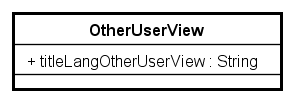
\includegraphics[scale=0.80]{UML/Classi/Front-End/QuizziPedia_Front-end_Views_OtherUserView.png}
	\caption{QuizziPedia::Front-End::Views::OtherUserView}
\end{figure} \FloatBarrier
\begin{itemize}
	\item \textbf{Descrizione}: view contenente le direttive dei dati personali e delle statistiche di un utente ricercato;
	\item \textbf{Utilizzo}: viene visualizzata dopo la ricerca e permette all'utente che ha l'ha effettuata di visualizzare i dati personali e le statistiche di un utente ricercato;
	\item \textbf{Relazioni con altre classi}:
	\begin{itemize}
		\item \textit{IN} \texttt{StatisticsDirective}: directive che permette di visualizzare le statistiche di un utente;
		\item \textit{IN} \texttt{UserDetailsDirective}: directive che permette di visualizzare i dati personali di un utente;
		\item \textit{IN} \texttt{LangModel}: rappresenta il modello delle informazioni per la giusta traduzione dell'applicazione.
	\end{itemize}
	\item \textbf{Attributi}:
	\begin{itemize}
		\item \texttt{+ titleLang: String} \\ Attributo che viene utilizzato per visualizzare la giusta traduzione del titolo della pagina, in italiano o in inglese.
	\end{itemize}
\end{itemize}


\paragraph{QuizziPedia::Front-End::Views::ProfileManagementView}
\begin{figure} [ht]
	\centering
	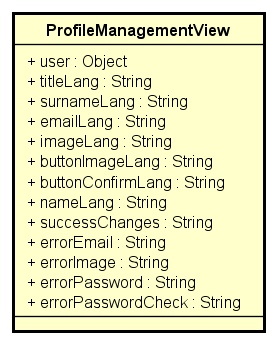
\includegraphics[scale=0.80]{UML/Classi/Front-End/QuizziPedia_Front-end_Views_ProfileManagementView.png}
	\caption{QuizziPedia::Front-End::Views::ProfileManagementView}
\end{figure} \FloatBarrier
\begin{itemize}
	\item \textbf{Descrizione}: view contenente i dati personali che un utente può modificare dopo essersi registrato al sistema;
	\item \textbf{Utilizzo}: permette all'utente di modificare tutti i campi elencati, tranne l'username, e di rendere persistenti tali modifiche se sono accettate dal sistema;
	\item \textbf{Relazioni con altre classi}:
	\begin{itemize}
		\item \textit{IN} \texttt{ProfileManagementController}: questa classe permette di gestire il profilo personale di un utente;
		\item \textit{IN} \texttt{ProfileManagementModelView}: classe di tipo modelview la cui istanzazione è contenuta all'interno della variabile di ambiente \$scope di \texttt{Angular.js}. All'interno di essa sono presenti le variabili e i metodi necessari per il \textit{Two-Way Data-Binding\ped{G}} tra la view \texttt{ProfileManagementView} e il controller \texttt{ProfileManagementController};
		\item \textit{IN} \texttt{LangModel}: rappresenta il modello delle informazioni per la giusta traduzione dell'applicazione.
	\end{itemize}
	\item \textbf{Attributi}:
	\begin{itemize}
		\item \texttt{+ user: Object} \\ Campo dati contenente i seguenti attributi: \texttt{name}, \texttt{surname}, \texttt{email}, \texttt{image}, \texttt{password} e \texttt{passwordCheck};
		\item \texttt{+ titleLang: String} \\ Attributo che viene utilizzato per visualizzare la giusta traduzione del titolo della pagina, in italiano o in inglese;
		\item \texttt{+ nameLang: String} \\ Attributo che viene utilizzato per visualizzare la giusta traduzione della \textit{label\ped{G}} per l'inserimento del nome, in italiano o in inglese;
		\item \texttt{+ surnameLang: String} \\ Attributo che viene utilizzato per visualizzare la giusta traduzione della \textit{label\ped{G}} per l'inserimento del cognome, in italiano o in inglese;
		\item \texttt{+ emailLang: String} \\ Attributo che viene utilizzato per visualizzare la giusta traduzione della \textit{label\ped{G}} per l'inserimento della posta elettronica, in italiano o in inglese;
		\item \texttt{+ imageLang: String} \\ Attributo che viene utilizzato per visualizzare la giusta traduzione della \textit{label\ped{G}} per l'inserimento dell'immagine, in italiano o in inglese;
		\item \texttt{+ buttonImageLang: String} \\ Attributo che viene utilizzato per visualizzare la giusta traduzione della \textit{label\ped{G}} per il bottone di caricamento immagine, in italiano o in inglese;
		\item \texttt{+ buttonConfirmLang: String} \\ Attributo che viene utilizzato per visualizzare la giusta traduzione della \textit{label\ped{G}} per il bottone di conferma, in italiano o in inglese;
		\item \texttt{+ successChanges: String} \\ Attributo che visualizza un messaggio di conferma avvenute modifiche;
		\item \texttt{+ errorEmail: String} \\ Attributo che visualizza un eventuale messaggio di errore nell'inserimento della email;
		\item \texttt{+ errorImage: String} \\ Attributo che visualizza un eventuale messaggio di errore nell'inserimento dell'immagine;
		\item \texttt{+ errorPassword: String} \\ Attributo che visualizza un eventuale messaggio di errore nell'inserimento della password;
		\item \texttt{+ errorPasswordCheck: String} \\ Attributo che visualizza un eventuale messaggio di errore nell'inserimento della password di conferma.
	\end{itemize}
\end{itemize}


\paragraph{QuizziPedia::Front-End::Views::QuestionsManagementView}
\begin{figure} [ht]
	\centering
	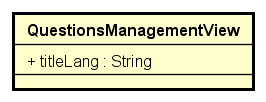
\includegraphics[scale=0.80]{UML/Classi/Front-End/QuizziPedia_Front-end_Views_QuestionsManagementView.png}
	\caption{QuizziPedia::Front-End::Views::QuestionsManagementView}
\end{figure} \FloatBarrier
\begin{itemize}
	\item \textbf{Descrizione}: view contenente l'elenco delle domande create; 
	\item \textbf{Utilizzo}: visualizza l'elenco delle domande create permettendo all'utente di crearne una nuova o di modificarne una presente nell'elenco;
	\item \textbf{Relazioni con altre classi}:
	\begin{itemize} 
		\item \textit{IN} \texttt{QuestionsManagementController}: questa classe permette di gestire le domande create dall'utente e di crearne di nuove;
		\item \textit{IN} \texttt{QuestionsManagementModelView}: classe di tipo modelview la cui istanzazione è contenuta all'interno della variabile di ambiente \$scope di \texttt{Angular.js}. All'interno di essa sono presenti le variabili e i metodi necessari per il \textit{Two-Way Data-Binding\ped{G}} tra la view \texttt{QuestionsManagementView} e il controller \texttt{QuestionsManagementController};
		\item \textit{IN} \texttt{OneQuestionDirective}: rappresenta il componente grafico che visualizza all'utente l'anteprima della domanda che ha creato. Eseguendo l'azione di click su di essa sarà possibile modificare tale domanda. All'interno di QuestionsManagementsView verranno stampati a video tanti componenti quanti presenti nello \$scope isolato ad esso associato;
		\item \textit{IN} \texttt{NewQuestionButtonDirective}:  rappresenta il componente grafico che permette all'utente di posizionarsi nella view di creazione di una nuova domanda;
		\item \textit{IN} \texttt{LangModel}: rappresenta il modello delle informazioni per la giusta traduzione dell'applicazione. 
	\end{itemize}
	\item \textbf{Attributi}:
	\begin{itemize}
		\item \texttt{+ titleLang: String} \\ Attributo che viene utilizzato per visualizzare la giusta traduzione del titolo della pagina, in italiano o in inglese.
	\end{itemize}
\end{itemize}


\paragraph{QuizziPedia::Front-End::Views::TrueFalseQuestionsView}
\begin{figure} [ht]
	\centering
	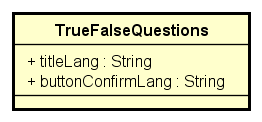
\includegraphics[scale=0.80]{UML/Classi/Front-End/QuizziPedia_Front-end_Views_TrueFalseQuestionsView.png}
	\caption{QuizziPedia::Front-End::Views::TrueFalseQuestionsView}
\end{figure} \FloatBarrier
\begin{itemize}
	\item \textbf{Descrizione}: view contenente le direttive per creare una domanda vero/falso; 
	\item \textbf{Utilizzo}: permette all'utente di creare una domanda vero/falso compilando i campi proposti;
	\item \textbf{Relazioni con altre classi}:
	\begin{itemize}
		\item \textit{IN} \texttt{TrueFalseQuestionsController}: questa classe permette di gestire la creazione e la modifica di una domanda vero/falso;
		\item \textit{IN} \texttt{TrueFalseQuestionsModelView}: classe di tipo modelview la cui istanzazione è contenuta all'interno della variabile di ambiente \$scope di \texttt{Angular.js}. All'interno di essa sono presenti le variabili e i metodi necessari per il \textit{Two-Way Data-Binding\ped{G}} tra la view \texttt{TrueFalseQuestionsView} e il controller \texttt{TrueFalseQuestionsController};
		\item \textit{IN} \texttt{TopicKeywordsDirective}: directive che permette di gestire l'inserimento di keywords al momento della creazione della domanda;
		\item \textit{IN} \texttt{ImageInTheQuestionDirective}: directive per l'inserimento dell'immagine nella creazione delle domande;
		\item \textit{IN} \texttt{QuestionTextDirective}: rappresenta il componente grafico che permette all'utente di scrivere o modificare il testo di una domanda;
		\item \textit{IN} \texttt{AnswerChoiceDirective}: directive contenente il componente grafico per le risposte a scelta;  
		\item \textit{IN} \texttt{LangModel}: rappresenta il modello delle informazioni per la giusta traduzione dell'applicazione.
	\end{itemize}
\item \textbf{Attributi}:
	\begin{itemize}
		\item \texttt{+ titleLang: String} \\ Attributo che viene utilizzato per visualizzare la giusta traduzione del titolo della pagina, in italiano o in inglese;
		\item \texttt{+ buttonConfirmLang: String} \\ Attributo che viene utilizzato per visualizzare la giusta traduzione della \textit{label\ped{G}} per il bottone di conferma, in italiano o in inglese;
		\item \texttt{+ successCreation: String} \\ Attributo che visualizza un messaggio di conferma avvenuta creazione della domanda;
		\item \texttt{+ errorCreation: String} \\ Attributo che visualizza un messaggio d'errore per la creazione della domanda.
	\end{itemize}
\end{itemize}


\paragraph{QuizziPedia::Front-End::Views::MultipleQuestionsView}
\begin{figure} [ht]
	\centering
	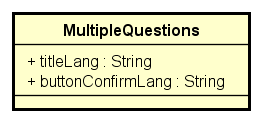
\includegraphics[scale=0.80]{UML/Classi/Front-End/QuizziPedia_Front-end_Views_MultipleQuestionsView.png}
	\caption{QuizziPedia::Front-End::Views::MultipleQuestionsView}
\end{figure} \FloatBarrier
\begin{itemize}
	\item \textbf{Descrizione}: view contenente le direttive per creare una domanda a risposta multipla;
	\item \textbf{Utilizzo}: permette all'utente di creare una domanda a risposta multipla compilando i campi proposti;
	\item \textbf{Relazioni con altre classi}:
		\begin{itemize}
			\item \textit{IN} \texttt{MultipleQuestionsController}: questa classe permette di gestire la creazione e la modifica di una domanda a risposta multipla;
			\item \textit{IN} \texttt{MultipleQuestionsModelView}: classe di tipo modelview la cui istanzazione è contenuta all'interno della variabile di ambiente \$scope di \texttt{Angular.js}. All'interno di essa sono presenti le variabili e i metodi necessari per il \textit{Two-Way Data-Binding\ped{G}} tra la view \texttt{MultipleQuestionsView} e il controller \texttt{MultipleQuestionsController};
			\item \textit{IN} \texttt{TopicKeywordsDirective}: directive che permette di gestire l'inserimento di keywords al momento della creazione della domanda;
			\item \textit{IN} \texttt{ImageInTheQuestionDirective}: directive per l'inserimento dell'immagine nella creazione delle domande;
			\item \textit{IN} \texttt{QuestionTextDirective}: rappresenta il componente grafico che permette all'utente di scrivere o modificare il testo di una domanda;
			\item \textit{IN} \texttt{AnswerChoiceDirective}: directive contenente il componente grafico per le risposte a scelta;
			\item \textit{IN} \texttt{LangModel}: rappresenta il modello delle informazioni per la giusta traduzione dell'applicazione.
		\end{itemize}
	\item \textbf{Attributi}:
	\begin{itemize}
		\item \texttt{+ titleLang: String} \\ Attributo che viene utilizzato per visualizzare la giusta traduzione del titolo della pagina, in italiano o in inglese;
		\item \texttt{+ buttonConfirmLang: String} \\ Attributo che viene utilizzato per visualizzare la giusta traduzione della \textit{label\ped{G}} per il bottone di conferma, in italiano o in inglese;
		\item \texttt{+ buttonLoadImageLang: String} \\ Attributo che viene utilizzato per visualizzare la giusta traduzione della \textit{label\ped{G}} per il bottone di caricamento dell'immagine nel testo della domanda, in italiano o in inglese;
		\item \texttt{+ successCreation: String} \\ Attributo che visualizza un messaggio di conferma avvenuta creazione della domanda;
		\item \texttt{+ errorCreation: String} \\ Attributo che visualizza un messaggio d'errore per la creazione della domanda.
	\end{itemize}
\end{itemize}


\paragraph{QuizziPedia::Front-End::Views::ConnectionQuestionsView}
\begin{figure} [ht]
	\centering
	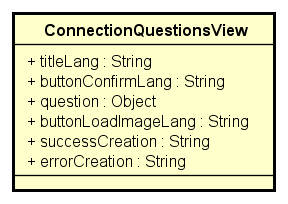
\includegraphics[scale=0.80]{UML/Classi/Front-End/QuizziPedia_Front-end_Views_ConnectionQuestionsView.png}
	\caption{QuizziPedia::Front-End::Views::ConnectionQuestionsView}
\end{figure} \FloatBarrier
\begin{itemize}
	\item \textbf{Descrizione}: view contenente i campi e le direttive per creare una domanda a collegamento;
	\item \textbf{Utilizzo}: permette all'utente di creare una domanda a collegamento compilando i campi proposti;
	\item \textbf{Relazioni con altre classi}:
	\begin{itemize}
		\item \textit{IN} \texttt{ConnectionQuestionsController}: questa classe permette di gestire la creazione e la modifica di una domanda a collegamento;
		\item \textit{IN} \texttt{ConnectionQuestionsModelView}: classe di tipo modelview la cui istanzazione è contenuta all'interno della variabile di ambiente \$scope di \texttt{Angular.js}. All'interno di essa sono presenti le variabili e i metodi necessari per il \textit{Two-Way Data-Binding\ped{G}} tra la view \texttt{ConnectionQuestionsView} e il controller \texttt{ConnectionQuestionsController};
		\item \textit{IN} \texttt{InputToListModelView}: classe di tipo modelview la cui istanzazione è contenuta all'interno della variabile di ambiente \$scope di \texttt{Angular.js}. All'interno di essa sono presenti le variabili e i metodi necessari per il \textit{Two-Way Data-Binding\ped{G}} tra la view \texttt{ConnectionQuestionsView} e il controller \texttt{InputToListController};
		\item \textit{IN} \texttt{TopicKeywordsDirective}: directive che permette di gestire l'inserimento di keywords al momento della creazione della domanda;
		\item \textit{IN} \texttt{QuestionTextDirective}: rappresenta il componente grafico che permette all'utente di scrivere o modificare il testo di una domanda;
		\item \textit{IN} \texttt{LangModel}: rappresenta il modello delle informazioni per la giusta traduzione dell'applicazione.
	\end{itemize}
	\item \textbf{Attributi}:
	\begin{itemize}
		\item \texttt{+ question: Object} \\ Oggetto contenente gli attributi per la creazione della domanda:
		\begin{itemize}
			\item \texttt{answer}: array contenente oggetti che rappresentano le risposte. Ogni oggetto risposta contiene:
			\begin{itemize}
				\item \texttt{text1}: di tipo \texttt{String}, rappresenta il primo elemento testuale che sarà collegato ad un secondo elemento (testuale o immagine);
				\item \texttt{text2}:  di tipo \texttt{String}, rappresenta il secondo elemento testuale che sarà collegato al primo elemento (testuale o immagine);
				\item \texttt{url1}: di tipo \texttt{String}, rappresenta il primo elemento immagine che sarà collegato con il secondo elemento (testuale o immagine);
				\item \texttt{url2}: di tipo \texttt{String}, rappresenta il secondo elemento immagine che sarà collegato con il primo elemento (testuale o immagine).
			\end{itemize}
		\end{itemize}			
		\item \texttt{+ titleLang: String} \\ Attributo che viene utilizzato per visualizzare la giusta traduzione del titolo della pagina, in italiano o in inglese;
		\item \texttt{+ buttonConfirmLang: String} \\ Attributo che viene utilizzato per visualizzare la giusta traduzione della \textit{label\ped{G}} per il bottone di conferma, in italiano o in inglese;
		\item \texttt{+ buttonLoadImageLang: String} \\ Attributo che viene utilizzato per visualizzare la giusta traduzione della \textit{label\ped{G}} per il bottone di caricamento dell'immagine nel testo della domanda, in italiano o in inglese;
		\item \texttt{+ successCreation: String} \\ Attributo che visualizza un messaggio di conferma avvenuta creazione della domanda;
		\item \texttt{+ errorCreation: String} \\ Attributo che visualizza un messaggio d'errore per la creazione della domanda.
	\end{itemize}
\end{itemize}


\paragraph{QuizziPedia::Front-End::Views::ImagesSortingQuestionsView}
\begin{figure} [ht]
	\centering
	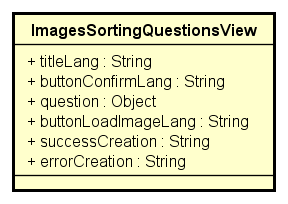
\includegraphics[scale=0.80]{UML/Classi/Front-End/QuizziPedia_Front-end_Views_ImagesSortingQuestionsView.png}
	\caption{QuizziPedia::Front-End::Views::ImagesSortingQuestionsView}
\end{figure} \FloatBarrier
\begin{itemize}
	\item \textbf{Descrizione}: view contenente i campi e le direttive per creare una domanda a ordinamento immagini;
	\item \textbf{Utilizzo}: permette all'utente di creare una domanda a ordinamento immagini compilando i campi proposti;
	\item \textbf{Relazioni con altre classi}:
	\begin{itemize}
		\item \textit{IN} \texttt{ImagesSortingQuestionsController}: questa classe permette di gestire la creazione e la modifica di una domanda a ordinamento immagini;
		\item \textit{IN} \texttt{ImageSortingQuestionsModelView}: classe di tipo modelview la cui istanzazione è contenuta all'interno della variabile di ambiente \$scope di \texttt{Angular.js}. All'interno di essa sono presenti le variabili e i metodi necessari per il \textit{Two-Way Data-Binding\ped{G}} tra la view \texttt{ImagesSortingQuestionsModelView} e il controller \texttt{ImagesSortingQuestionsController};
		\item \textit{IN} \texttt{InputToListModelView}: classe di tipo modelview la cui istanzazione è contenuta all'interno della variabile di ambiente \$scope di \texttt{Angular.js}. All'interno di essa sono presenti le variabili e i metodi necessari per il \textit{Two-Way Data-Binding\ped{G}} tra la view \texttt{ImageSortingQuestionsView} e il controller \texttt{InputToListController};
		\item \textit{IN} \texttt{ImageInTheQuestionDirective}: directive per l'inserimento dell'immagine nella creazione delle domande;
		\item \textit{IN} \texttt{TopicKeywordsDirective}: directive che permette di gestire l'inserimento di keywords al momento della creazione della domanda;
		\item \textit{IN} \texttt{QuestionTextDirective}: rappresenta il componente grafico che permette all'utente di scrivere o modificare il testo di una domanda;
		\item \textit{IN} \texttt{LangModel}: rappresenta il modello delle informazioni per la giusta traduzione dell'applicazione.
	\end{itemize}
	\item \textbf{Attributi}:
	\begin{itemize}
			\item \texttt{+ question: Object} \\ Oggetto contenente gli attributi per la creazione della domanda:
			\begin{itemize}
				\item \texttt{answer}: array contenente oggetti che rappresentano le risposte. Ogni oggetto risposta contiene:
				\begin{itemize}
					\item \texttt{urlSorting}: attributo di tipo \texttt{String} che contiene l'\textit{URL\ped{G}} dell'immagine associata alla risposta;
					\item \texttt{position}: attributo di tipo \texttt{Number} che indica la giusta posizione dell'immagine.
				\end{itemize}
			\end{itemize}	  
		\item \texttt{+ titleLang: String} \\ Attributo che viene utilizzato per visualizzare la giusta traduzione del titolo della pagina, in italiano o in inglese;
		\item \texttt{+ buttonConfirmLang: String} \\ Attributo che viene utilizzato per visualizzare la giusta traduzione della \textit{label\ped{G}} per il bottone di conferma, in italiano o in inglese;
		\item \texttt{+ buttonLoadImageLang: String} \\ Attributo che viene utilizzato per visualizzare la giusta traduzione della \textit{label\ped{G}} per il bottone di caricamento dell'immagine nel testo della domanda, in italiano o in inglese;
		\item \texttt{+ successCreation: String} \\ Attributo che visualizza un messaggio di conferma avvenuta creazione della domanda;
		\item \texttt{+ errorCreation: String} \\ Attributo che visualizza un messaggio d'errore per la creazione della domanda.
	\end{itemize}
\end{itemize}


\paragraph{QuizziPedia::Front-End::Views::StringsSortingQuestionsView}
\begin{figure} [ht]
	\centering
	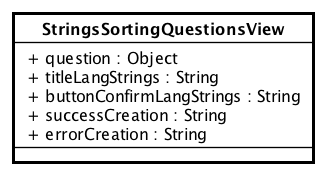
\includegraphics[scale=0.80]{UML/Classi/Front-End/QuizziPedia_Front-end_Views_StringsSortingQuestionsView.png}
	\caption{QuizziPedia::Front-End::Views::StringsSortingQuestionsView}
\end{figure} \FloatBarrier
\begin{itemize}
	\item \textbf{Descrizione}: view contenente i campi e le direttive per creare una domanda a ordinamento stringhe;
	\item \textbf{Utilizzo}: permette all'utente di creare una domanda a ordinamento stringhe compilando i campi proposti;
	\item \textbf{Relazioni con altre classi}:
		\begin{itemize}
			\item \textit{IN} \texttt{StringsSortingQuestionsController}: questa classe permette di gestire la creazione e la modifica di una domanda a ordinamento di stringhe;
			\item \textit{IN} \texttt{StringsSortingQuestionsModelView}: classe di tipo modelview la cui istanzazione è contenuta all'interno della variabile di ambiente \$scope di \texttt{Angular.js}. All'interno di essa sono presenti le variabili e i metodi necessari per il \textit{Two-Way Data-Binding\ped{G}} tra la view \texttt{StringsSortingQuestionsView} e il controller \texttt{StringsSortingQuestionsController};
			\item \textit{IN} \texttt{InputToListModelView}: classe di tipo modelview la cui istanzazione è contenuta all'interno della variabile di ambiente \$scope di \texttt{Angular.js}. All'interno di essa sono presenti le variabili e i metodi necessari per il \textit{Two-Way Data-Binding\ped{G}} tra la view \texttt{StringsSortingQuestionsView} e il controller \texttt{InputToListController};
			\item \textit{IN} \texttt{TopicKeywordsDirective}: directive che permette di gestire l'inserimento di keywords al momento della creazione della domanda;
			\item \textit{IN} \texttt{QuestionTextDirective}: rappresenta il componente grafico che permette all'utente di scrivere o modificare il testo di una domanda;
			\item \textit{IN} \texttt{LangModel}: rappresenta il modello delle informazioni per la giusta traduzione dell'applicazione.
		\end{itemize}
	\item \textbf{Attributi}:
	\begin{itemize}
		\item \texttt{+ question: Object} \\ Oggetto contenente gli attributi per la creazione della domanda:
		\begin{itemize}
			\item \texttt{answer}: array contenente oggetti che rappresentano le risposte. Ogni oggetto risposta contiene:
			\begin{itemize}
				\item \texttt{textSorting}: attributo di tipo \texttt{String} che contiene il testo della risposta;
				\item \texttt{position}: attributo di tipo \texttt{Number} che indica la giusta posizione del testo.
			\end{itemize}
		\end{itemize}	  
		\item \texttt{+ titleLang: String} \\ Attributo che viene utilizzato per visualizzare la giusta traduzione del titolo della pagina, in italiano o in inglese;
		\item \texttt{+ buttonConfirmLang: String} \\ Attributo che viene utilizzato per visualizzare la giusta traduzione della \textit{label\ped{G}} per il bottone di conferma, in italiano o in inglese;
		\item \texttt{+ successCreation: String} \\ Attributo che visualizza un messaggio di conferma avvenuta creazione della domanda;
		\item \texttt{+ errorCreation: String} \\ Attributo che visualizza un messaggio d'errore per la creazione della domanda.
	\end{itemize}
\end{itemize}


\paragraph{QuizziPedia::Front-End::Views::FillingQuestionsView}
\begin{figure} [ht]
	\centering
	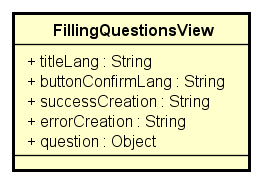
\includegraphics[scale=0.80]{UML/Classi/Front-End/QuizziPedia_Front-end_Views_FillingQuestionsView.png}
	\caption{QuizziPedia::Front-End::Views::FillingQuestionsView}
\end{figure} \FloatBarrier
\begin{itemize}
	\item \textbf{Descrizione}: view contenente i campi e le direttive per creare una domanda a riempimento testo;
	\item \textbf{Utilizzo}:  permette all'utente di creare una domanda a riempimento testo compilando i campi proposti;
	\item \textbf{Relazioni con altre classi}:
	\begin{itemize}
		\item \textit{IN} \texttt{FillingQuestionsController}: questa classe permette di gestire la creazione e la modifica di una domanda a riempimento di spazi;
		\item \textit{IN} \texttt{FillingQuestionsModelView}: classe di tipo modelview la cui istanzazione è contenuta all'interno della variabile di ambiente \$scope di \texttt{Angular.js}. All'interno di essa sono presenti le variabili e i metodi necessari per il \textit{Two-Way Data-Binding\ped{G}} tra la view \texttt{FillingQuestionsView} e il controller \texttt{FillingQuestionsController};
		\item \textit{IN} \texttt{TopicKeywordsDirective}: directive che permette di gestire l'inserimento di keywords al momento della creazione della domanda;
		\item \textit{IN} \texttt{QuestionTextDirective}: rappresenta il componente grafico che permette all'utente di scrivere o modificare il testo di una domanda;
		\item \textit{IN} \texttt{LangModel}: rappresenta il modello delle informazioni per la giusta traduzione dell'applicazione.
	\end{itemize}
	\item \textbf{Attributi}:
	\begin{itemize}
		\item \texttt{+ question: Object} \\ Oggetto contenente gli attributi per la creazione della domanda:
		\begin{itemize}
			\item \texttt{answer}: array contenente oggetti che rappresentano le risposte. Ogni oggetto risposta contiene:
				\begin{itemize}
					\item \texttt{wordNumber}: attributo di tipo \texttt{Number} che indica la parola nel testo che andrà inserita in fase di compilazione.
				\end{itemize}
		\end{itemize}
		\item \texttt{+ titleLang: String} \\ Attributo che viene utilizzato per visualizzare la giusta traduzione del titolo della pagina, in italiano o in inglese;
		\item \texttt{+ buttonConfirmLang: String} \\ Attributo che viene utilizzato per visualizzare la giusta traduzione della \textit{label\ped{G}} per il bottone di conferma, in italiano o in inglese;
		\item \texttt{+ successCreation: String} \\ Attributo che visualizza un messaggio di conferma avvenuta creazione della domanda;
		\item \texttt{+ errorCreation: String} \\ Attributo che visualizza un messaggio d'errore per la creazione della domanda.
	\end{itemize}
\end{itemize}


\paragraph{QuizziPedia::Front-End::Views::ClickableAreaQuestionsView}
\begin{figure} [ht]
	\centering
	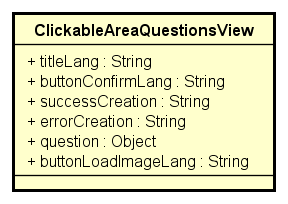
\includegraphics[scale=0.80]{UML/Classi/Front-End/QuizziPedia_Front-end_ClickableAreaQuestionsView.png}
	\caption{QuizziPedia::Front-End::Views::ClickableAreaQuestionsView}
\end{figure} \FloatBarrier
\begin{itemize}
	\item \textbf{Descrizione}: view contenente i campi e le direttive per creare una domanda ad area cliccabile;
	\item \textbf{Utilizzo}:  permette all'utente di creare una domanda ad area cliccabile compilando i campi proposti;
	\item \textbf{Relazioni con altre classi}:
	\begin{itemize}
		\item \textit{IN} \texttt{ClickableAreaQuestionsController}: questa classe permette di gestire la creazione e la modifica di una domanda ad area cliccabile;
		\item \textit{IN} \texttt{ClickableAreaQuestionsModelView}: classe di tipo modelview la cui istanzazione è contenuta all'interno della variabile di ambiente \$scope di \texttt{Angular.js}. All'interno di essa sono presenti le variabili e i metodi necessari per il \textit{Two-Way Data-Binding\ped{G}} tra la view \texttt{ClickableAreaQuestionsView} e il controller \texttt{ClickableAreaQuestionsController};
		\item \textit{IN} \texttt{TopicKeywordsDirective}: directive che permette di gestire l'inserimento di keywords al momento della creazione della domanda;
		\item \textit{IN} \texttt{QuestionTextDirective}: rappresenta il componente grafico che permette all'utente di scrivere o modificare il testo di una domanda;
		\item \textit{IN} \texttt{LangModel}: rappresenta il modello delle informazioni per la giusta traduzione dell'applicazione.
	\end{itemize}
	\item \textbf{Attributi}:
	\begin{itemize}
		\item \texttt{+ question: Object} \\ Oggetto contenente gli attributi per la creazione della domanda:
		\begin{itemize}
			\item \texttt{url}: attributo di tipo \texttt{String} che contiene l'\textit{URL\ped{G}} associato all'immagine;
			\item \texttt{answer}: array contenente oggetti che rappresentano le risposte. Ogni oggetto risposta contiene:
			\begin{itemize}
				\item \texttt{x}: attributo di tipo \texttt{Number} che rappresenta la posizione della risposta nell'asse delle ascisse all'interno dell'immagine;
				\item \texttt{y}: attributo di tipo \texttt{Number} che rappresenta la posizione della risposta nell'asse delle ordinate all'interno dell'immagine.
			\end{itemize}
		\end{itemize}	
		\item \texttt{+ titleLang: String} \\ Attributo che viene utilizzato per visualizzare la giusta traduzione del titolo della pagina, in italiano o in inglese;
		\item \texttt{+ buttonConfirmLang: String} \\ Attributo che viene utilizzato per visualizzare la giusta traduzione della \textit{label\ped{G}} per il bottone di conferma, in italiano o in inglese;
		\item \texttt{+ buttonLoadImageLang: String} \\ Attributo che viene utilizzato per visualizzare la giusta traduzione della \textit{label\ped{G}} per il bottone di caricamento dell'immagine nel testo della domanda, in italiano o in inglese;
		\item \texttt{+ successCreation: String} \\ Attributo che visualizza un messaggio di conferma avvenuta creazione della domanda;
		\item \texttt{+ errorCreation: String} \\ Attributo che visualizza un messaggio d'errore per la creazione della domanda.
	\end{itemize}
\end{itemize}


\paragraph{QuizziPedia::Front-End::Views::EditorQMLView}
\begin{figure} [ht]
	\centering
	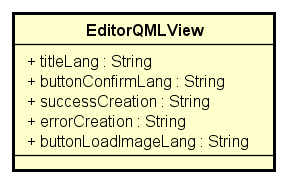
\includegraphics[scale=0.80]{UML/Classi/Front-End/QuizziPedia_Front-end_EditorQMLView.png}
	\caption{QuizziPedia::Front-End::Views::EditorQMLView}
\end{figure} \FloatBarrier
\begin{itemize}
	\item \textbf{Descrizione}: view contenente l'editor QML per la creazione di domande personalizzate;
	\item \textbf{Utilizzo}: permette ad un utente di creare domande personalizzate attraverso la scrittura del codice QML direttamente nell'editor di testo presente nella view;
	\item \textbf{Relazioni con altre classi}:
	\begin{itemize}
		\item \textit{IN} \texttt{EditorQMLController}: questa classe permette di gestire la creazione e la modifica di domande create tramite editor QML;
		\item \textit{IN} \texttt{EditorQMLModelView}: classe di tipo modelview la cui istanzazione è contenuta all'interno della variabile di ambiente \$scope di \texttt{Angular.js}. All'interno di essa sono presenti le variabili e i metodi necessari per il \textit{Two-Way Data-Binding\ped{G}} tra la view \texttt{EditorQMLView} e il controller \texttt{EditorQMLController};
		\item \textit{IN} \texttt{LangModel}: rappresenta il modello delle informazioni per la giusta traduzione dell'applicazione.
	\end{itemize}
	\item \textbf{Attributi}:
	\begin{itemize}
		\item \texttt{+ titleLang: String} \\ Attributo che viene utilizzato per visualizzare la giusta traduzione del titolo della pagina, in italiano o in inglese;
		\item \texttt{+ buttonConfirmLang: String} \\ Attributo che viene utilizzato per visualizzare la giusta traduzione della \textit{label\ped{G}} per il bottone di conferma, in italiano o in inglese;
		\item \texttt{+ buttonLoadImageLang: String} \\ Attributo che viene utilizzato per visualizzare la giusta traduzione della \textit{label\ped{G}} per il bottone di caricamento dell'immagine nel testo della domanda, in italiano o in inglese;
		\item \texttt{+ successCreation: String} \\ Attributo che visualizza un messaggio di conferma avvenuta creazione della domanda;
		\item \texttt{+ errorCreation: String} \\ Attributo che visualizza un messaggio d'errore per la creazione della domanda.
	\end{itemize}
\end{itemize}

\paragraph{QuizziPedia::Front-End::Views::TrainingView}
\begin{figure} [ht]
	\centering
	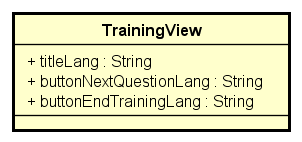
\includegraphics[scale=0.80]{UML/Classi/Front-End/QuizziPedia_Front-end_TrainingView.png}
	\caption{QuizziPedia::Front-End::Views:TrainingView}
\end{figure} \FloatBarrier
\begin{itemize}
	\item \textbf{Descrizione}: view principale della modalità allenamento; conterrà i vari templates di ogni domanda dell'allenamento;
	\item \textbf{Utilizzo}: all'interno di essa verrà caricato inizialmente il template dove si potranno scegliere l'argomento e le parole chiave dell'allenamento; verranno poi caricati i templates di ogni domanda in base alle preferenze scelte; 
	\item \textbf{Relazioni con altre classi}:
	\begin{itemize}
		\item \textit{IN} \texttt{TrainingController}: questa classe permette di gestire la modalità allenamento sottoponendo all'utente le giuste domande adatte al suo livello;
		\item \textit{IN} \texttt{TrainingModelView}: classe di tipo modelview la cui istanzazione è contenuta all'interno della variabile di ambiente \$scope di \texttt{Angular.js}. All'interno di essa sono presenti le variabili e i metodi necessari per il \textit{Two-Way Data-Binding\ped{G}} tra la view \texttt{TrainingView} e il controller \texttt{TrainingController};
		\item \textit{IN} \texttt{TrainingSetUpDirective}: rappresenta il componente grafico che permette all'utente di selezionare l'argomento e le parole chiave per iniziare un allenamento con queste caratteristiche. Viene visualizzato	dinamicamente all'interno delle views TrainingView e FillingQuestionnaireView mediante il controller QuestionsController;
		\item \textit{IN} \texttt{HeaderTextQuestionDirective}:rappresenta il componente grafico che presenta all'utente il testo della domanda, l'argomento e le parole chiave. Viene visualizzato dinamicamente all'interno delle views TrainingView e FillingQuestionnaireView mediante il controller QuestionsController;
		\item \textit{IN} \texttt{TrueFalseAnswerDirective}: rappresenta il componente grafico che permette all'utente di visualizzare la domanda vero e falso. Viene visualizzato dinamicamente all'interno delle views TrainingView e FillingQuestionnaireView mediante il controller QuestionsController;
		\item \textit{IN} \texttt{MultipleChoiceAnswerDirective}: rappresenta il componente grafico che permette all'utente di visualizzare la domanda a risposta multipla. Viene visualizzato dinamicamente all'interno delle views TrainingView e FillingQuestionnaireView mediante il controller QuestionsController;
		\item \textit{IN} \texttt{LinkingAnswerDirective}: rappresenta il componente grafico che permette all'utente di visualizzare la domanda di collegamento. Viene visualizzato dinamicamente all'interno delle views TrainingView e FillingQuestionnaireView mediante il controller QuestionsController;
		\item \textit{IN} \texttt{SortImagesAnswerDirective}: rappresenta il componente grafico che permette all'utente di visualizzare la domanda ad ordinamento di immagini. Viene visualizzato dinamicamente all'interno delle views TrainingView e FillingQuestionnaireView mediante il controller QuestionsController;
		\item \textit{IN} \texttt{SortTextAnswerDirective}: rappresenta il componente grafico che permette all'utente di visualizzare la domanda ad ordinamento di stringhe. Viene visualizzato dinamicamente all'interno delle views TrainingView e FillingQuestionnaireView mediante il controller QuestionsController;
		\item \textit{IN} \texttt{EmptySpaceAnswerDirective}: rappresenta il componente grafico che permette all'utente di visualizzare l'esercizio a riempimento di spazi vuoti. Viene visualizzato dinamicamente all'interno delle views TrainingView e FillingQuestionnaireView mediante il controller QuestionsController;
		\item \textit{IN} \texttt{ClickableAnswerDirective}: rappresenta il componente grafico che permette all'utente di visualizzare la domanda ad area cliccabile nell'immagine. Viene visualizzato dinamicamente all'interno delle views TrainingView e FillingQuestionnaireView mediante il controller QuestionsController;
		\item \textit{IN} \texttt{LangModel}: rappresenta il modello delle informazioni per la giusta traduzione dell'applicazione.
	\end{itemize}
	\item \textbf{Attributi}:
	\begin{itemize}
		\item \texttt{+ titleLang: String} \\ Attributo che viene utilizzato per visualizzare la giusta traduzione del titolo della pagina, in italiano o in inglese;
		\item \texttt{+ buttonNextQuestionLang: String} \\ Attributo che viene utilizzato per visualizzare la giusta traduzione della \textit{label\ped{G}} per il bottone di avanzamento a domanda successiva, in italiano o in inglese;
		\item \texttt{+ buttonEndTrainingLang: String} \\ Attributo che viene utilizzato per visualizzare la giusta traduzione della \textit{label\ped{G}} per il bottone di conclusione dell'allenamento, in italiano o in inglese.
	\end{itemize}
\end{itemize}


\paragraph{QuizziPedia::Front-End::Views::FillingQuestionnaireView}
\begin{figure} [ht]
	\centering
	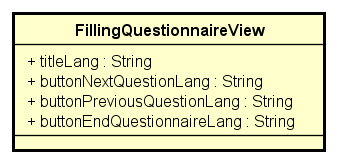
\includegraphics[scale=0.80]{UML/Classi/Front-End/QuizziPedia_Front-end_FillingQuestionnaireView.png}
	\caption{QuizziPedia::Front-End::Views:FillingQuestionnaireView}
\end{figure} \FloatBarrier
\begin{itemize}
	\item \textbf{Descrizione}: view principale per la compilazione del questionario; conterrà i vari templates di ogni domanda appartenente al questionario;
	\item \textbf{Utilizzo}: all'interno di essa verrà caricato inizialmente il template contenente le informazioni generali relative al questionario; verranno poi caricati i templates di ogni domanda presente nel questionario;
	\item \textbf{Relazioni con altre classi}: 
	\begin{itemize}
		\item \textit{IN} \texttt{FillingQuestionnaireController}: questa classe permette di gestire la compilazione del questionario;
		\item \textit{IN} \texttt{FillingQuestionnaireModelView}: classe di tipo modelview la cui istanzazione è contenuta all'interno della variabile di ambiente \$scope di \texttt{Angular.js}. All'interno di essa sono presenti le variabili e i metodi necessari per il \textit{Two-Way Data-Binding\ped{G}} tra la view \texttt{FillingQuestionnaireView} e il controller \texttt{FillingQuestionnaireController};
		\item \textit{IN} \texttt{InfoQuestionnaireDirective}: rappresenta il componente grafico che permette all'utente di visualizzare le informazioni principali del questionario che si sta per svolgere. Viene visualizzato dinamicamente all'interno delle views TrainingView e FillingQuestionnaireView mediante il controller QuestionsController;
		\item \textit{IN} \texttt{HeaderTextQuestionDirective}:rappresenta il componente grafico che presenta all'utente il testo della domanda, l'argomento e le parole chiave. Viene visualizzato dinamicamente all'interno delle views TrainingView e FillingQuestionnaireView mediante il controller QuestionsController;
		\item \textit{IN} \texttt{TrueFalseAnswerDirective}: rappresenta il componente grafico che permette all'utente di visualizzare la domanda vero e falso. Viene visualizzato dinamicamente all'interno delle views TrainingView e FillingQuestionnaireView mediante il controller QuestionsController;
		\item \textit{IN} \texttt{MultipleChoiceAnswerDirective}: rappresenta il componente grafico che permette all'utente di visualizzare la domanda a risposta multipla. Viene visualizzato dinamicamente all'interno delle views TrainingView e FillingQuestionnaireView mediante il controller QuestionsController;
		\item \textit{IN} \texttt{LinkingAnswerDirective}: rappresenta il componente grafico che permette all'utente di visualizzare la domanda di collegamento. Viene visualizzato dinamicamente all'interno delle views TrainingView e FillingQuestionnaireView mediante il controller QuestionsController;
		\item \textit{IN} \texttt{SortImagesAnswerDirective}: rappresenta il componente grafico che permette all'utente di visualizzare la domanda ad ordinamento di immagini. Viene visualizzato dinamicamente all'interno delle views TrainingView e FillingQuestionnaireView mediante il controller QuestionsController;
		\item \textit{IN} \texttt{SortTextAnswerDirective}: rappresenta il componente grafico che permette all'utente di visualizzare la domanda ad ordinamento di stringhe. Viene visualizzato dinamicamente all'interno delle views TrainingView e FillingQuestionnaireView mediante il controller QuestionsController;
		\item \textit{IN} \texttt{EmptySpaceAnswerDirective}: rappresenta il componente grafico che permette all'utente di visualizzare l'esercizio a riempimento di spazi vuoti. Viene visualizzato dinamicamente all'interno delle views TrainingView e FillingQuestionnaireView mediante il controller QuestionsController;
		\item \textit{IN} \texttt{ClickableAnswerDirective}: rappresenta il componente grafico che permette all'utente di visualizzare la domanda ad area cliccabile nell'immagine. Viene visualizzato dinamicamente all'interno delle views TrainingView e FillingQuestionnaireView mediante il controller QuestionsController;
		\item \textit{IN} \texttt{LangModel}: rappresenta il modello delle informazioni per la giusta traduzione dell'applicazione.
	\end{itemize}
		\item \textbf{Attributi}:
		\begin{itemize}
			\item \texttt{+ titleLang: String} \\ Attributo che viene utilizzato per visualizzare la giusta traduzione del titolo della pagina, in italiano o in inglese;
			\item \texttt{+ buttonNextQuestionLang: String} \\ Attributo che viene utilizzato per visualizzare la giusta traduzione della \textit{label\ped{G}} per il bottone di avanzamento a domanda successiva, in italiano o in inglese;
			\item \texttt{+ buttonPreviousQuestionLang: String} \\ Attributo che viene utilizzato per visualizzare la giusta traduzione della \textit{label\ped{G}} per il bottone di ritorno alla domanda precedente, in italiano o in inglese;
			\item \texttt{+ buttonEndQuestionnaireLang: String} \\ Attributo che viene utilizzato per visualizzare la giusta traduzione della \textit{label\ped{G}} per il bottone di conclusione del questionario, in italiano o in inglese. 
		\end{itemize}
\end{itemize}


\paragraph{QuizziPedia::Front-End::Views::QuestionnaireManagementView}
\begin{figure} [ht]
	\centering
	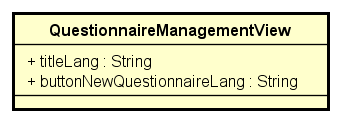
\includegraphics[scale=0.80]{UML/Classi/Front-End/QuizziPedia_Front-end_QuestionnaireManagementView.png}
	\caption{QuizziPedia::Front-End::Views:QuestionnaireManagementView}
\end{figure} \FloatBarrier
\begin{itemize}
	\item \textbf{Descrizione}: view principale per la gestione dei questionari;
	\item \textbf{Utilizzo}: permette di visualizzare tutti i questionari creati, quelli abilitati per la compilazione e quelli non ancora abilitati; contiene inoltre il link per la creazione di un nuovo questionario;
	\item \textbf{Relazioni con altre classi}:
	\begin{itemize}
		\item \textit{IN} \texttt{QuestionnaireManagementController}: questa classe permette di gestire tutti i questionari creati da un utente;
		\item \textit{IN} \texttt{QuestionnaireManagementModelView}: classe di tipo modelview la cui istanzazione è contenuta all'interno della variabile di ambiente \$scope di \texttt{Angular.js}. All'interno di essa sono presenti le variabili e i metodi necessari per il \textit{Two-Way Data-Binding\ped{G}} tra la view \texttt{QuestionnaireManagementView} e il controller \texttt{QuestionnaireManagementController};
		\item \textit{IN} \texttt{EliminationAndModifyDirective}: direttiva contenente i componenti grafici  che permettono di eliminare un questionario o di modificarne uno esistente;
		\item \textit{IN} \texttt{ExamModalityDirective}: directive contenete i componenti grafici per attivare la modalità esame su un questionario e gestire le iscrizioni;
		\item \textit{IN} \texttt{QuestionnaireResultsDirective}: rappresenta il componente grafico che permette all'utente autenticato pro di vedere i risultati di chi ha compilato il questionario. Tale componente è contenuto nella lista dei questionari abilitati alla compilazione. \'E possibile accedere alla lista dei risultati azionando l'evento ad esso collegato;
		\item \textit{IN} \texttt{LangModel}: rappresenta il modello delle informazioni per la giusta traduzione dell'applicazione.
	\end{itemize}
		\item \textbf{Attributi}:
		\begin{itemize}
			\item \texttt{+ titleLang: String} \\ Attributo che viene utilizzato per visualizzare la giusta traduzione del titolo della pagina, in italiano o in inglese;
			\item \texttt{+ questionnaireList: Array} \\ Array contenente la lista dei questionari creati; ogni questionario sarà rappresentato come un oggetto;
			\item \texttt{+ buttonNewQuestionnaireLang: String} \\ Attributo che viene utilizzato per visualizzare la giusta traduzione della \textit{label\ped{G}} per il bottone di creazione di un nuovo questionario, in italiano o in inglese.
		\end{itemize}
\end{itemize}


\paragraph{QuizziPedia::Front-End::Views::CreateQuestionnaireView}
\begin{figure} [ht]
	\centering
	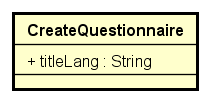
\includegraphics[scale=0.80]{UML/Classi/Front-End/QuizziPedia_Front-end_CreateQuestionnaireView.png}
	\caption{QuizziPedia::Front-End::Views:CreateQuestionnaireView}
\end{figure} \FloatBarrier
\begin{itemize}
	\item \textbf{Descrizione}: view per la creazione del questionario. In questo componente viene permesso anche all'utente di:
	\begin{itemize}
		\item Effettuare delle ricerche sul database di domande;
		\item Selezionare le domande da inserire nel questionario;
		\item Mostrare le domande già inserite e permettere all'utente di eliminarle da tale lista.
	\end{itemize}
	\item \textbf{Utilizzo}: permette all'utente di creare un questionario compilando tutti i campi proposti;
	\item \textbf{Relazioni con altre classi}:
	\begin{itemize}
		\item \textit{IN} \texttt{CreateQuestionnaireController}:  questa classe permette di gestire la creazione di un questionario;
		\item \textit{IN} \texttt{CreateQuestionnaireModelView}: classe di tipo modelview la cui istanzazione è contenuta all'interno della variabile di ambiente \$scope di \texttt{Angular.js}. All'interno di essa sono presenti le variabili e i metodi necessari per il \textit{Two-Way Data-Binding\ped{G}} tra la view \texttt{CreateQuestionnaireView} e il controller \texttt{CreateQuestionnaireController};
<<<<<<< HEAD
		\item \textit{IN} \texttt{KeywordsDirective}: directive che permette di gestire l'inserimento dell'argomento e delle keywords al momento della creazione della domanda;
=======
		\item \textit{IN} \texttt{TopicKeywordsDirective}: directive che permette di gestire l'inserimento dell'argomento e delle keywords al momento della creazione della domanda;
		\item \textit{IN} \texttt{QuestionsManagementQuestionnaireDirective}: rappresenta il componente grafico che permette all'utente di:
		\begin{itemize}
			\item Effettuare delle ricerche sul database di domande;
			\item Selezionare le domande da inserire nel questionario;
			\item Mostrare le domande già inserite e permettere all'utente di eliminarle da tale lista.
		\end{itemize}
>>>>>>> ed1574a720d7cc95292367f7465ea9f90fa08128
		\item \textit{IN} \texttt{LangModel}: rappresenta il modello delle informazioni per la giusta traduzione dell'applicazione.
	\end{itemize}
		\item \textbf{Attributi}:
		\begin{itemize}
			\item \texttt{+ nameQuestionnaire: String}: \\ Attributo che specifica il nome del questionario creato;
			\item \texttt{+ titleLang: String} \\ Attributo che viene utilizzato per visualizzare la giusta traduzione del titolo della pagina, in italiano o in inglese;
			\item \texttt{+ buttonConfirmLang: String} \\ Attributo che viene utilizzato per visualizzare la giusta traduzione della \textit{label\ped{G}} per il bottone di conferma, in italiano o in inglese;
			\item \texttt{+ successCreation: String} \\ Attributo che visualizza un messaggio di conferma avvenuta creazione della domanda;
			\item \texttt{+ errorCreation: String} \\ Attributo che visualizza un messaggio d'errore per la creazione della domanda.
			\item \texttt{+ question: String} \\ Attributo che conterrà la stringa per la ricerca della domanda;
			\item \texttt{+ questions: Array} \\ Array contenente le domande trovate durante la ricerca;
			\item \texttt{+ pushButton: String} \\ Attributo che viene utilizzato per visualizzare la giusta traduzione della \textit{label\ped{G}} per il bottone di inserimento delle domande selezionate, in italiano o in inglese;
			\item \texttt{+ deleteButton: String} \\ Attributo che viene utilizzato per visualizzare la giusta traduzione della \textit{label\ped{G}} per il bottone di eliminazione delle domande dal questionario, in italiano o in inglese;
		\end{itemize}
\end{itemize}


\paragraph{QuizziPedia::Front-End::Views::RegistrationManagementView}
\begin{figure} [ht]
	\centering
	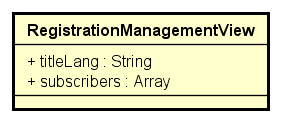
\includegraphics[scale=0.80]{UML/Classi/Front-End/QuizziPedia_Front-end_RegistrationManagementView.png}
	\caption{QuizziPedia::Front-End::Views:RegistrationManagementView}
\end{figure} \FloatBarrier
\begin{itemize}
	\item \textbf{Descrizione}: view per la gestione degli utenti iscritti a un proprio questionario;
	\item \textbf{Utilizzo}: permette di visualizzare tutti gli utenti iscritti al proprio questionario e abilitarli alla compilazione;
	\item \textbf{Relazioni con altre classi}:
	\begin{itemize}
		\item \textit{IN} \texttt{RegistrationManagementController}: questa classe permette di gestire le iscrizione degli utenti ai questionari; 
		\item \textit{IN} \texttt{RegistratioManagementModelView}: classe di tipo modelview la cui istanzazione è contenuta all'interno della variabile di ambiente \$scope di \texttt{Angular.js}. All'interno di essa sono presenti le variabili e i metodi necessari per il \textit{Two-Way Data-Binding\ped{G}} tra la view \texttt{RegistrationManagementView} e il controller \texttt{RegistrationManagementController}; 
		\item \textit{IN} \texttt{LangModel}: rappresenta il modello delle informazioni per la giusta traduzione dell'applicazione.
	\end{itemize}
		\item \textbf{Attributi}:
		\begin{itemize}
			\item \texttt{+ titleLang: String} \\ Attributo che viene utilizzato per visualizzare la giusta traduzione del titolo della pagina, in italiano o in inglese; 
			\item \texttt{+ subscribers: Array} \\ Array contenete un oggetto per ogni utente iscritto al questionario. L'oggetto sarà composto dai campi \texttt{nome} e \texttt{cognome};
			\item \texttt{+ enableLangButton} \\ Attributo che viene utilizzato per visualizzare la giusta traduzione della \textit{label\ped{G}} per il bottone di abilitazione al questionario per un utente selezionato, in italiano o in inglese;
			\item \texttt{+ disableLangButton} \\ Attributo che viene utilizzato per visualizzare la giusta traduzione della \textit{label\ped{G}} per il bottone di non abilitazione al questionario per un utente selezionato, in italiano o in inglese.
		\end{itemize}
\end{itemize}


\paragraph{QuizziPedia::Front-End::Views::ResultsQuestionnarieView}
\begin{figure} [ht]
	\centering
	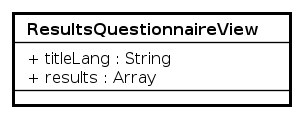
\includegraphics[scale=0.80]{UML/Classi/Front-End/QuizziPedia_Front-end_ResultsQuestionnarieView.png}
	\caption{QuizziPedia::Front-End::Views:ResultsQuestionnarieView}
\end{figure} \FloatBarrier
\begin{itemize}
	\item \textbf{Descrizione}: view contenente i risultati conseguiti dagli utenti che hanno compilato il proprio questionario;
	\item \textbf{Utilizzo}: permette di visualizzare i risultati di ogni utente conseguiti nella compilazione del questionario;
	\item \textbf{Relazioni con altre classi}:
	\begin{itemize}
		\item \textit{IN} \texttt{ResultsController}: questa classe permette di gestire i risultati della ricerca effettuata dall'utente;
		\item \textit{IN} \texttt{ResultsQuestionnaireModelView}: classe di tipo modelview la cui istanzazione è contenuta all'interno della variabile di ambiente \$scope di \texttt{Angular.js}. All'interno di essa sono presenti le variabili e i metodi necessari per il \textit{Two-Way Data-Binding\ped{G}} tra la view \texttt{ResultsQuestionnarieView} e il controller \texttt{ResultsController}; 
		\item \textit{IN} \texttt{LangModel}: rappresenta il modello delle informazioni per la giusta traduzione dell'applicazione.
	\end{itemize}
	\item \textbf{Attributi}:
	\begin{itemize}
		\item \texttt{+ titleLang: String} \\ Attributo che viene utilizzato per visualizzare la giusta traduzione del titolo della pagina, in italiano o in inglese; 
		\item \texttt{+ results: Array} \\ Array contenente un oggetto per ogni iscritto che ha compilato il questionario. L'oggetto sarà composto dai campi: \texttt{nome} e \texttt{cognome} e \texttt{valutazione}.
	\end{itemize}
\end{itemize}